\documentclass[dissertation.tex]{subfiles} 
\begin{document}

\chapter{Event Selection}
\label{chap:Event Selection}

In keeping with the phenomenology described in Sec.~\ref{sec:Phenomenology of General Gauge Mediation}, the candidate GGM events selected in this search consist of two high-$E_{T}$ photons and a significant momentum imbalance transverse to the beam, indicating the production of an escaping gravitino.  This momentum imbalance is usually referred to as \textit{missing transverse energy} and is denoted by the symbol \MET.

However, in order to use real CMS data (as opposed to simulation) to derive predictions for the backgrounds to the search, \textit{control samples} distinct from the \textit{candidate} two-photon sample must be collected.  These samples consist of different numerical combinations of photons, electrons, and jets, and are explained in more detail in Chapter~\ref{chap:Data Analysis}.  Since this search is performed in the high-\MET tail of the \MET distribution, where adequate detector simulation is very difficult, it is advantageous to use \textit{data-driven} background estimates, which capture the true detector response, over numbers derived from simulation.

In the following sections, the reconstruction of photons, electrons, jets, and \MET is explained.  Sec.~\ref{sec:Object Reconstruction} begins with an explanation of the high level reconstruction.  It is followed by Sec.~\ref{sec:HLT}, which describes the triggers used to collect the candidate and control samples.  Finally, the chapter concludes with a measurement of the photon identification efficiency in Sec.~\ref{sec:Photon Identification Efficiency}.

\section{Object Reconstruction}
\label{sec:Object Reconstruction}

This section describes the \textit{offline} object reconstruction, i.e. the reconstruction of particle objects from events that have already been triggered and written to permanent storage, as opposed to the building of trigger objects explained in Secs.~\ref{sec:Level 1 and High Level Trigger Systems} and~\ref{sec:HLT}.

\subsection{Photons}
\label{sec:Photons}

\subsubsection{Uncalibrated EB/EE Hits}
\label{sec:Uncalibrated EB/EE Hits}

Photon reconstruction begins with the ADC count value for each of the 10 recorded time samples per ECAL crystal per trigger.  To construct an \textit{uncalibrated hit}, the gain (1, 6, or 12; see Sec.~\ref{sec:Electromagnetic Calorimeter}) of each sample is determined and the ADC count value scaled appropriately.  The pedestal is estimated from the average of the first three samples, which, for a properly time in hit, should contain no signal.  This pedestal value is subtracted from the rest of the samples.  Finally, the amplitude of the pulse is reconstructed using a predetermined weight for each sample \cite{Bruneliere}.  The weights correspond to the pulse shape expected from the MGPA and shaping circuit response.  The time of the hit is also reconstructed using the ratios between neighboring time samples \cite{time_reco}.  A typical ECAL channel pulse shape is shown in Figure~\ref{fig:pulse}.

\begin{figure}
	\centering
	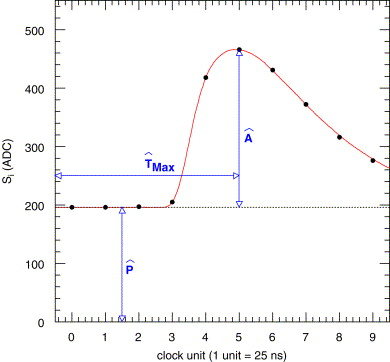
\includegraphics[scale=2.0]{pulse}
	\caption{Typical ECAL channel pulse shape.  $\widehat{P}$ is the pedestal value, $\widehat{A}$ is the pulse amplitude, and $\widehat{T}_{\mathrm{max}}$ is the hit time.  The red line is the assumed pulse shape from which the weights are derived.  Reprinted from ref. \cite{Bruneliere}.}
	\label{fig:pulse}
\end{figure}

\subsubsection{Calibrated EB/EE Hits}
\label{sec:Calibrated EB/EE Hits}

In the next phase of the photon reconstruction, calibrations are applied to the uncalibrated hits to form \textit{calibrated hits} with energy measured in GeV.  Channels are excluded from seeding calibrated hits if

\begin{itemize}
\item they are excessively noisy,
\item they are stuck in fixed gain,
\item they are totally dead,
\item they have one or more neighboring dead channels, or
\item they do not have good trigger primitives (i.e. trigger primitive is missing, saturated, or spike-like).
\end{itemize}
%
In addition, no uncalibrated hits that are spike-like are eligible for calibration.  The calibrations applied are crystal transparency loss corrections measured continuously by the laser/LED system, energy intercalibrations (relative energy calibration between crystals), absolute scale calibrations between ADC counts and GeV,\footnote{The ADC-GeV scale factors (one for EB and one for EE) are defined such that the sum of fully calibrated and scaled hits in a particular 5 $\times$ cluster of crystals (plus the associated energy deposited in ES) is 50 GeV for a 50 GeV incident unconverted photon \cite{calibration_IN}.} and time intercalibrations (relative time calibration between crystals).

%reference for EE lab intercalibrations?
The ECAL crystals were pre-calibrated before installation in CMS using laboratory light yield and photodetector gain measurements \cite{EB_performance_2006}.  In addition, some EB and EE crystals were intercalibrated using test beams \cite{EB_startup_intercalibration}, and all EB crystals were intercalibrated with cosmic ray muons \cite{CRAFT_calibration}.  EE precalibrations were validated with LHC \textit{splash events} in 2009 \cite{CRAFT_calibration, CRAFT_ECAL_performance}, in which the beam was dumped onto a collimator approximately 150 meters upstream of CMS, causing a spray of muons to enter CMS at one endcap and exit at the other.  Splash events were also used to derive time intercalibration constants.  Before colliding beam operations commenced, the intercalibration precision was estimated to be 0.5\%-2.2\% in EB and 1\%-5\% in EE \cite{CALOR_ECAL_calibration}.

Three calibration methods were employed once colliding beam operations began:

\begin{itemize}
\item $\phi$ symmetry relative calibration between crystals, exploiting the azimuthal symmetry of CMS
\item $\pi^{0}$ and $\eta$ relative calibration between crystals, using the diphoton decays of these particles
\item $E/p$ absolute calibration, comparing the momentum measured in the tracker $p$ to the energy measured in the ECAL $E$ of a sample of electrons from $Z$ decay
\end{itemize}
%
By September 2011, the intercalibration precision in EB was measured to be between 0.3\% and 1.1\% using the $\pi^{0}/\eta$ method \cite{Yang}.  Figure~\ref{fig:intercalibration} shows the improvement in $Z$ reconstruction from pre-LHC calibration constants to the latest $\pi^{0}/\eta$-derived constants.

\begin{figure}
	\centering
	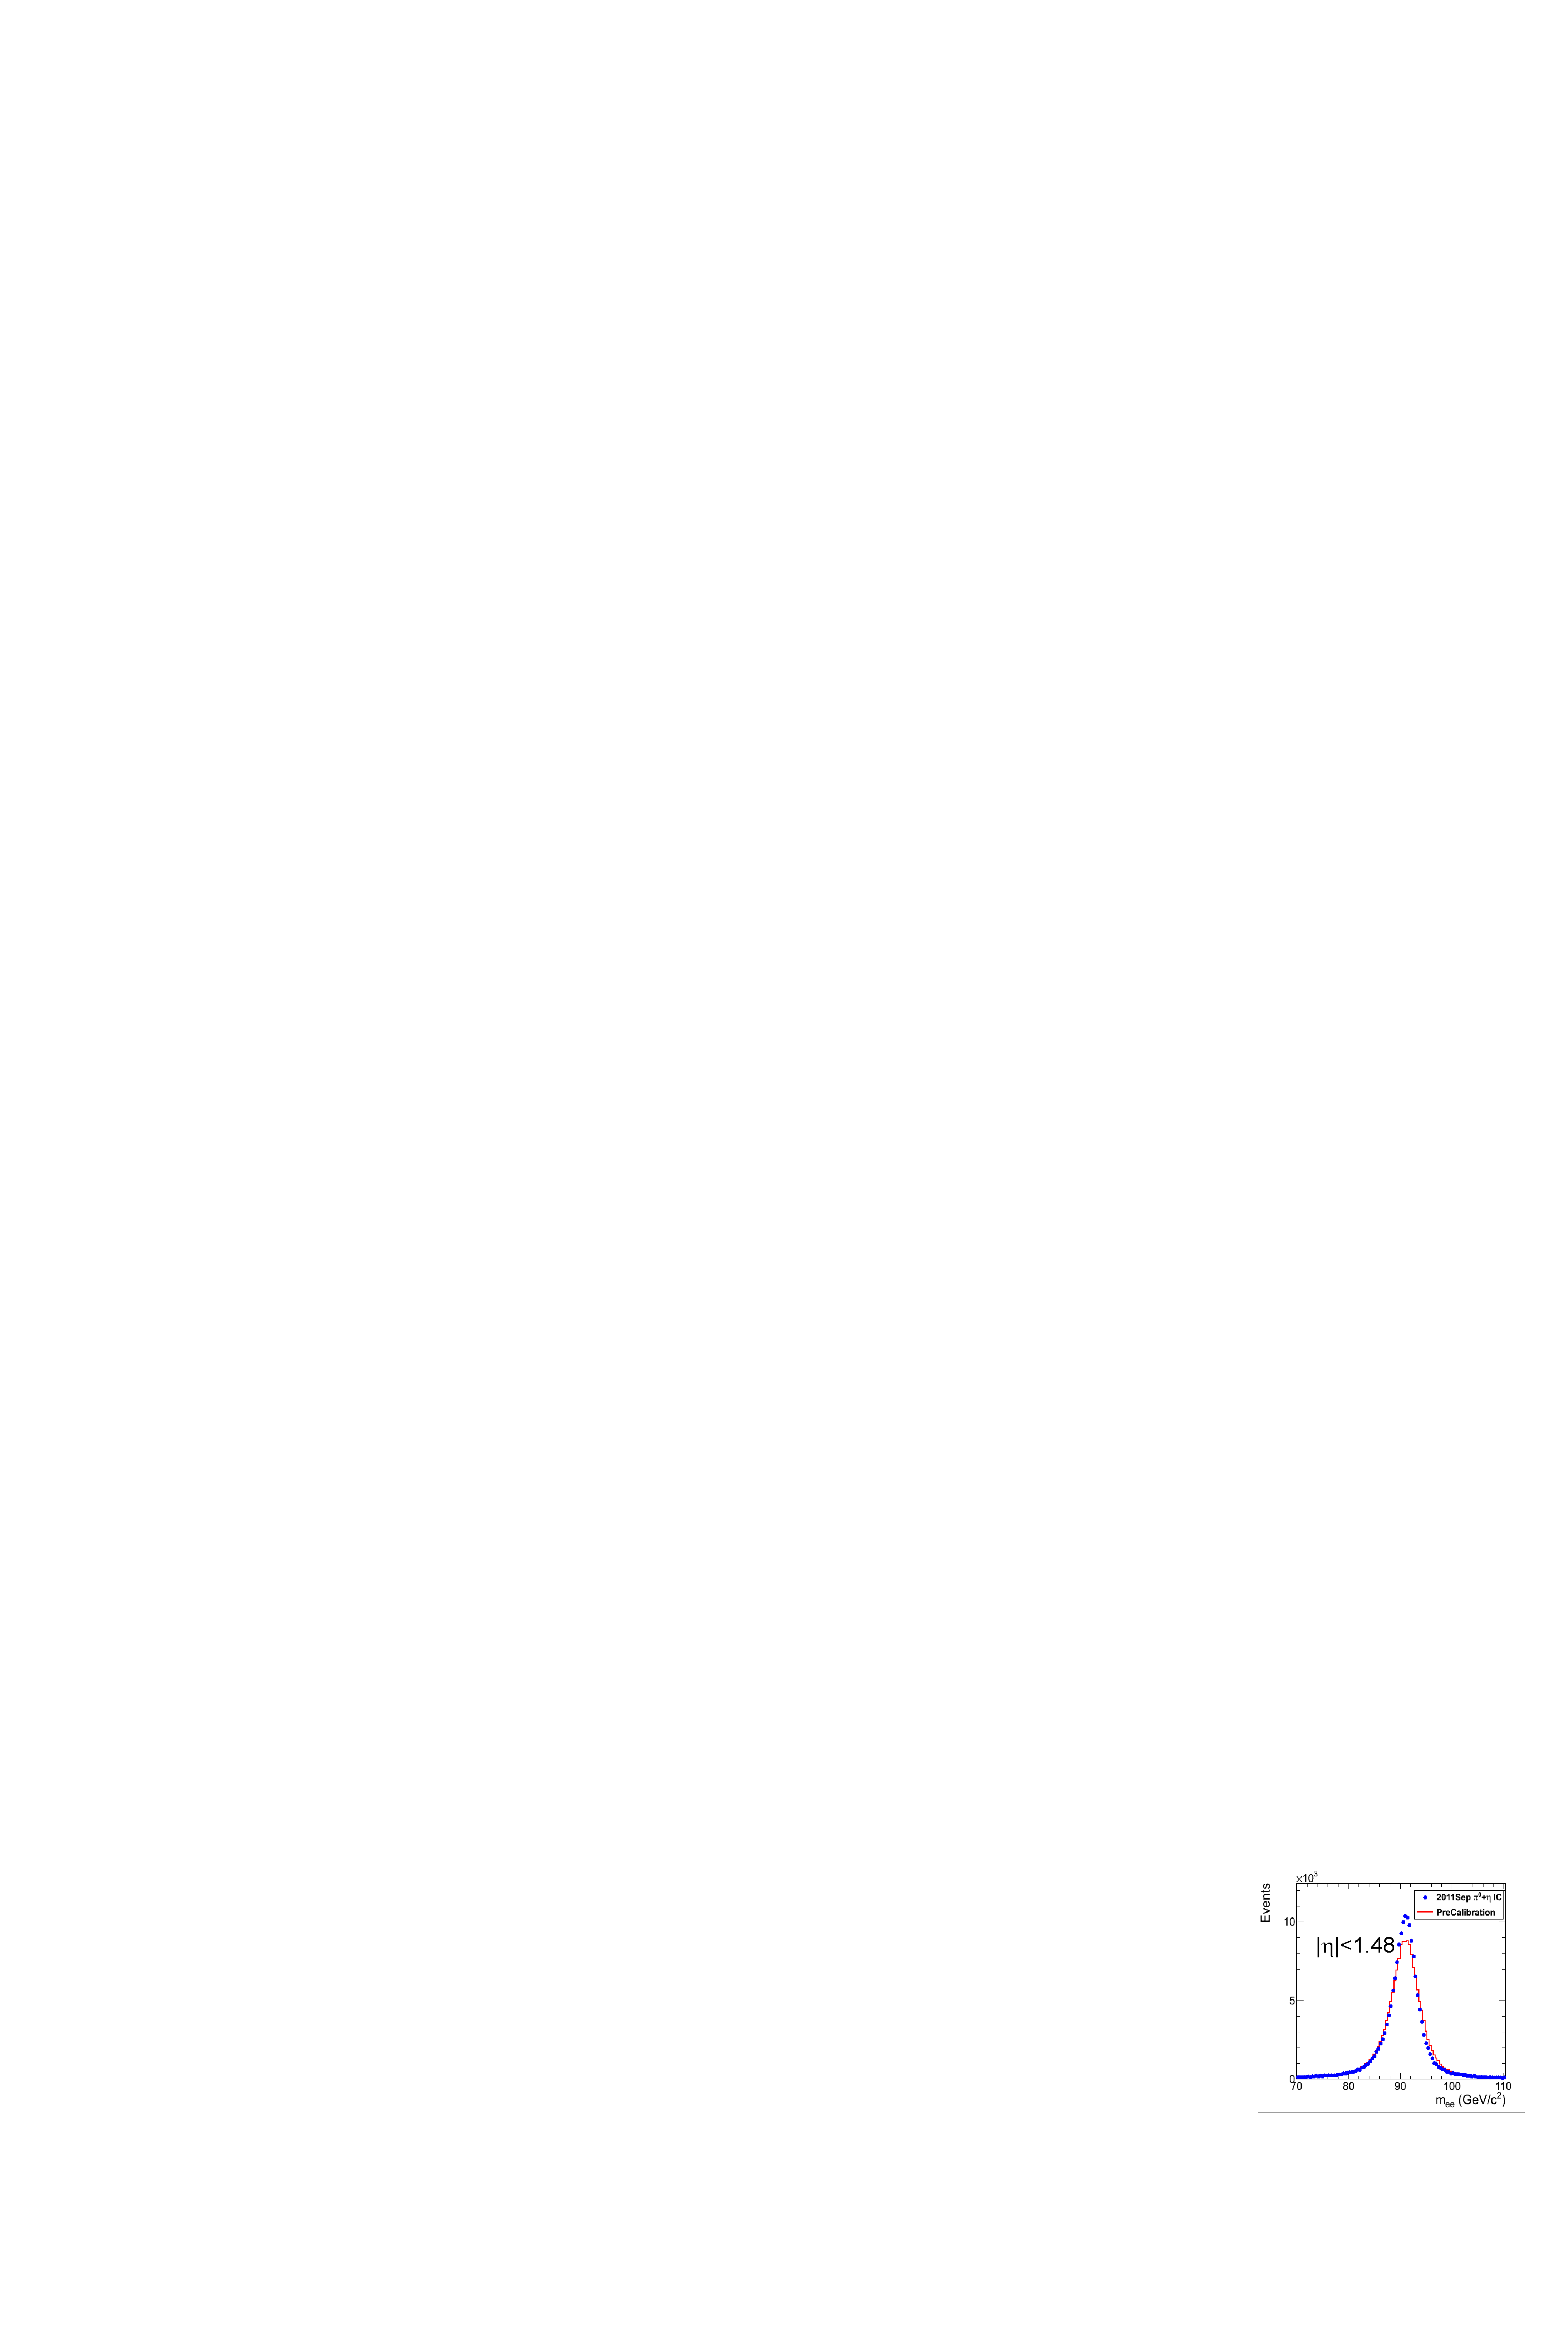
\includegraphics[scale=0.5]{intercalibration}
	\caption{$Z$ peak reconstructed using pre-LHC calibration constants (red) or September 2011 $\pi^{0}/\eta$-derived intercalibration constants (blue).  Reprinted from ref. \cite{Yang}.}
	\label{fig:intercalibration}
\end{figure}

\subsubsection{Calibrated ES Hits}
\label{sec:Calibrated ES Hits}

%what are angle correction constants?
ES calibrated hits are formed from the three samples read out per sensor.  Just as in the case of EB/EE crystals, ES uncalibrated hits gain-adjusted, pedestal-subtracted, and reconstructed using weights.  To make a calibrated ES hit, intercalibration constants, angle correction constants, and a MIP-GeV absolute scale factor are applied.

\subsubsection{Clustering}

After calibrated ECAL hits are formed, they must be clustered into shapes that represent the energy deposit from a single particle.  \textit{Basic clusters} are formed around seed hits, defined as a hit that

\begin{itemize}
\item has calibrated $E_{T} >$ 1(0.18) GeV in EB(EE),
\item does not originate from a dead channel or one with faulty hardware,
\item is not poorly calibrated,
\item was reconstructed with the standard algorithm (i.e. not a special recovery algorithm for channels with subpar data integrity),
\item is not saturated,
\item is not spike-like, and
\item is in time (EB).
\end{itemize}
%
EB basic clusters are formed around the seeds via the \textit{hybrid} algorithm, while EE basic clusters are formed with the \textit{multi5x5} algorithm \cite{ECAL_SC_note}.  In addition to non-radiating electrons and unconverted photons, both algorithms are designed to also recover all of the energy associated with electron bremsstrahlung deposits and photon conversions.  The geometry of the CMS magnetic field means that bremsstrahlung and conversions will tend to spread the shower out in $\phi$, not $\eta$.  Both algorithms work by forming basic clusters around seeds, then combining the basic clusters into \textit{superclusters} (SC) by searching in a window extended in the $\phi$ direction for all basic clusters consistent with bremsstrahlung radiation from the primary electron, or with a photon conversion.  Figure~\ref{fig:hybrid} illustrates the hybrid algorithm in EB.  In EE, the energy deposited in ES must also be added into the total clustered energy sum.

\begin{figure}
	\centering
	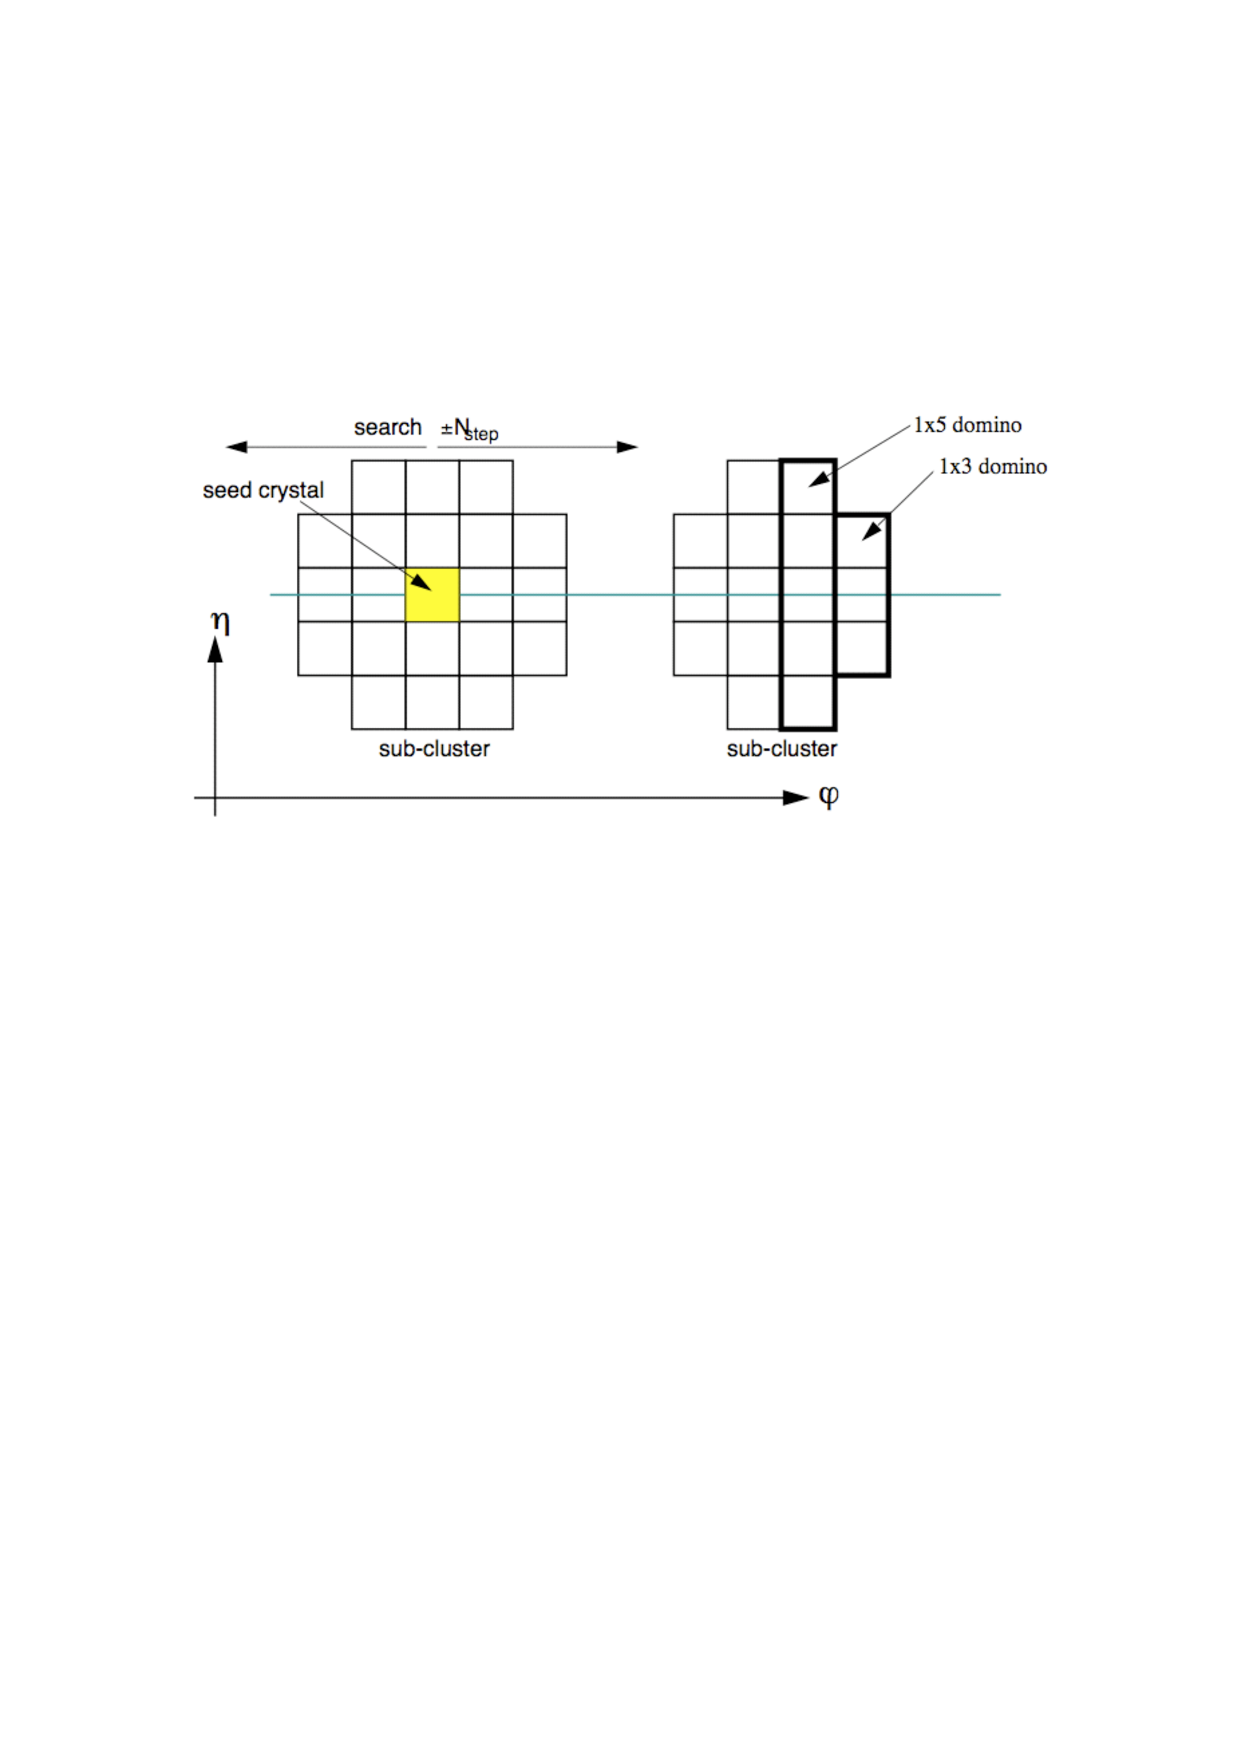
\includegraphics[scale=0.5]{hybrid}
	\caption{Hybrid algorithm in EB.  The shower extent is essentially constant in $\eta$, but spreads out in $\phi$ as the two sub-clusters (or basic clusters) are grouped into the same supercluster.  Reprinted from ref. \cite{ECAL_SC_note}.}
	\label{fig:hybrid}
\end{figure}

\subsubsection{Supercluster Corrections}
\label{sec:Supercluster Corrections}

The total clustered ECAL energy is defined as

\begin{eqnarray}
E &=& F \times \sum_{i=1}^{n_{\mathrm{crystal}}} G \times c_{i} \times A_{i}
\end{eqnarray}
%
where $G$ is the ADC-GeV or MIP-GeV scale factor, $c_{i}$ are the intercalibration constants, $A_{i}$ is the uncalibrated hit amplitude in ADC counts, and $F$ is SC correction factor.  $G$ and $c_{i}$ were explained in Secs.~\ref{sec:Calibrated EB/EE Hits} and~\ref{sec:Calibrated ES Hits}.  $F$ is a product of three factors for hybrid SCs (two for multi5x5 SCs) \cite{ECAL_SC_note}:

\begin{enumerate}
  %what exactly does this mean?
  \item $C_{EB}(\eta|)$, which compensates for lateral energy leakage due to the crystal off-pointing in EB.  These corrections are taken from MC simulation \cite{ECAL_SC_note} and were confirmed in test beams \cite{EB_startup_intercalibration}.
  \item $f(\mbox{brem})$, which corrects for the biases in the clustering algorithms for showers characterized by differing amounts of bremsstrahlung.  These corrections are taken from MC simulation \cite{ECAL_SC_note}.
  \item Residual correction $f(E_{T}, \eta)$, due to the variation in $\eta$ of detector material traversed by a primary electron or photon, and to any residual $E_{T}$ dependence of the reconstruction.  These corrections are determined from $Z\rightarrow ee$ data samples. %where is this documented?
\end{enumerate}

%best energy resolution, ideally in terms of stochastic, noise, and constant terms (e-mailed Doug)

\subsubsection{From Supercluster to Photon}
\label{sec:From Supercluster to Photon}

The CMS photon object is any SC with $E_{T} > 10$ GeV and $H/E < 0.5$, unless the SC $E_{T} > 100$ GeV, in which case the $H/E$ requirement is dropped.  $H/E$ is defined as the ratio of energy in the HCAL in a 0.15 cone around the SC centroid, directly behind the SC, to the SC energy.  SCs with $R9 > 0.94(0.95)$ in EB(EE), where $R9$ is defined as $E_{3\times 3}/E_{SC}$,  are the best calibrated and most accurate type of electromagnetic shower.  Therefore, for these objects, the photon energy is defined as the energy sum of the fully calibrated hits in the central 5 $\times$ 5 cluster around the seed (with $C_{EB}(\eta)$ applied for EB photons).  For all other SCs, the photon energy is equal to the fully corrected SC energy (cf. Sec.~\ref{sec:Supercluster Corrections}).

In this search, candidate photons and \textit{fake photons} ($\mathit{f}$, ``fakes") are further selected according to the criteria listed in Table~\ref{tab:g_f_criteria}.  Fakes are used in the determination of the QCD background, as explained in Chapter~\ref{chap:Data Analysis}.  $I_{\mathrm{comb}}$ is defined as

%fix with latest effective areas
\begin{eqnarray}
I_{\mathrm{comb}} &=& I_{\mathrm{ECAL}} - 0.0792\rho + I_{\mathrm{HCAL}} - 0.0252\rho + I_{\mathrm{track}}
\end{eqnarray}
%
where $I_{\mathrm{ECAL}}$, $I_{\mathrm{HCAL}}$, and $I_{\mathrm{track}}$ are $E_{T}$ sums in the annular regions defined in Figure~\ref{fig:isolation_cones} and $\rho$ is the average pileup energy density in the calorimeters (per unit $\eta\cdot\phi$) as measured with the Fastjet algorithm \cite{Fastjet_conf_proceedings, Fastjet_manual}.  Figure~\ref{fig:preselected_rho} shows the $\rho$ distribution for a sample of events with at least two 25 GeV EM objects passing the $|\eta|$, $H/E$, and $R9$ requirements in Table~\ref{g_f_criteria}, and passing the trigger requirements in Table~\ref{HLT_by_run_range}, representing the full 2011 dataset.  Since average $\rho$ is $\sim 5$ GeV, and there is a long tail above this average value, it is necessary to subtract pileup energy from the ECAL and HCAL isolation cones to recover otherwise clean photons in events with large pileup.  The ECAL and HCAL \textit{effective areas} of 0.0792 and 0.0252, respectively, are calculated by fitting the average ECAL or HCAL isolation energy vs. $\rho$ in a sample of $Z\rightarrow ee$ events to a straight line.  The slope of the line---which has the units of $\eta\cdot\phi$, or area---is the effective area.
%show Dave's rho plots?  make your own?

%define more precisely?
A ``pixel seed" is defined as a hit in the pixel detector consistent with a track extrapolated from the position of the ECAL SC back to the primary vertex.  Real photons, having no charge and therefore no bending in the magnetic field, should not have a pixel seed.

\begin{table}[hcbp]
\caption{Selection criteria for photons and fakes.}
\centering
\begin{tabular}{|c|c|c|}
\hline
Variable & Cut ($\gamma$) & Cut ($\mathit{f}$) \\
\hline
\hline
SC $|\eta|$ & $< 1.4442$ & $<1.4442$ \\
\hline
$H/E$ & $<0.05$ & $<0.05$ \\
\hline
$R9$ & $< 1$ & $< 1$ \\
\hline
Has pixel seed & No & No \\
\hline
$I_{\mathrm{comb}}$ & $< 6$ GeV & $\geq 6$ and $< 20$ GeV \\
\hline
\end{tabular}
\label{tab:g_f_criteria}
\end{table}

\begin{figure}
	\centering
	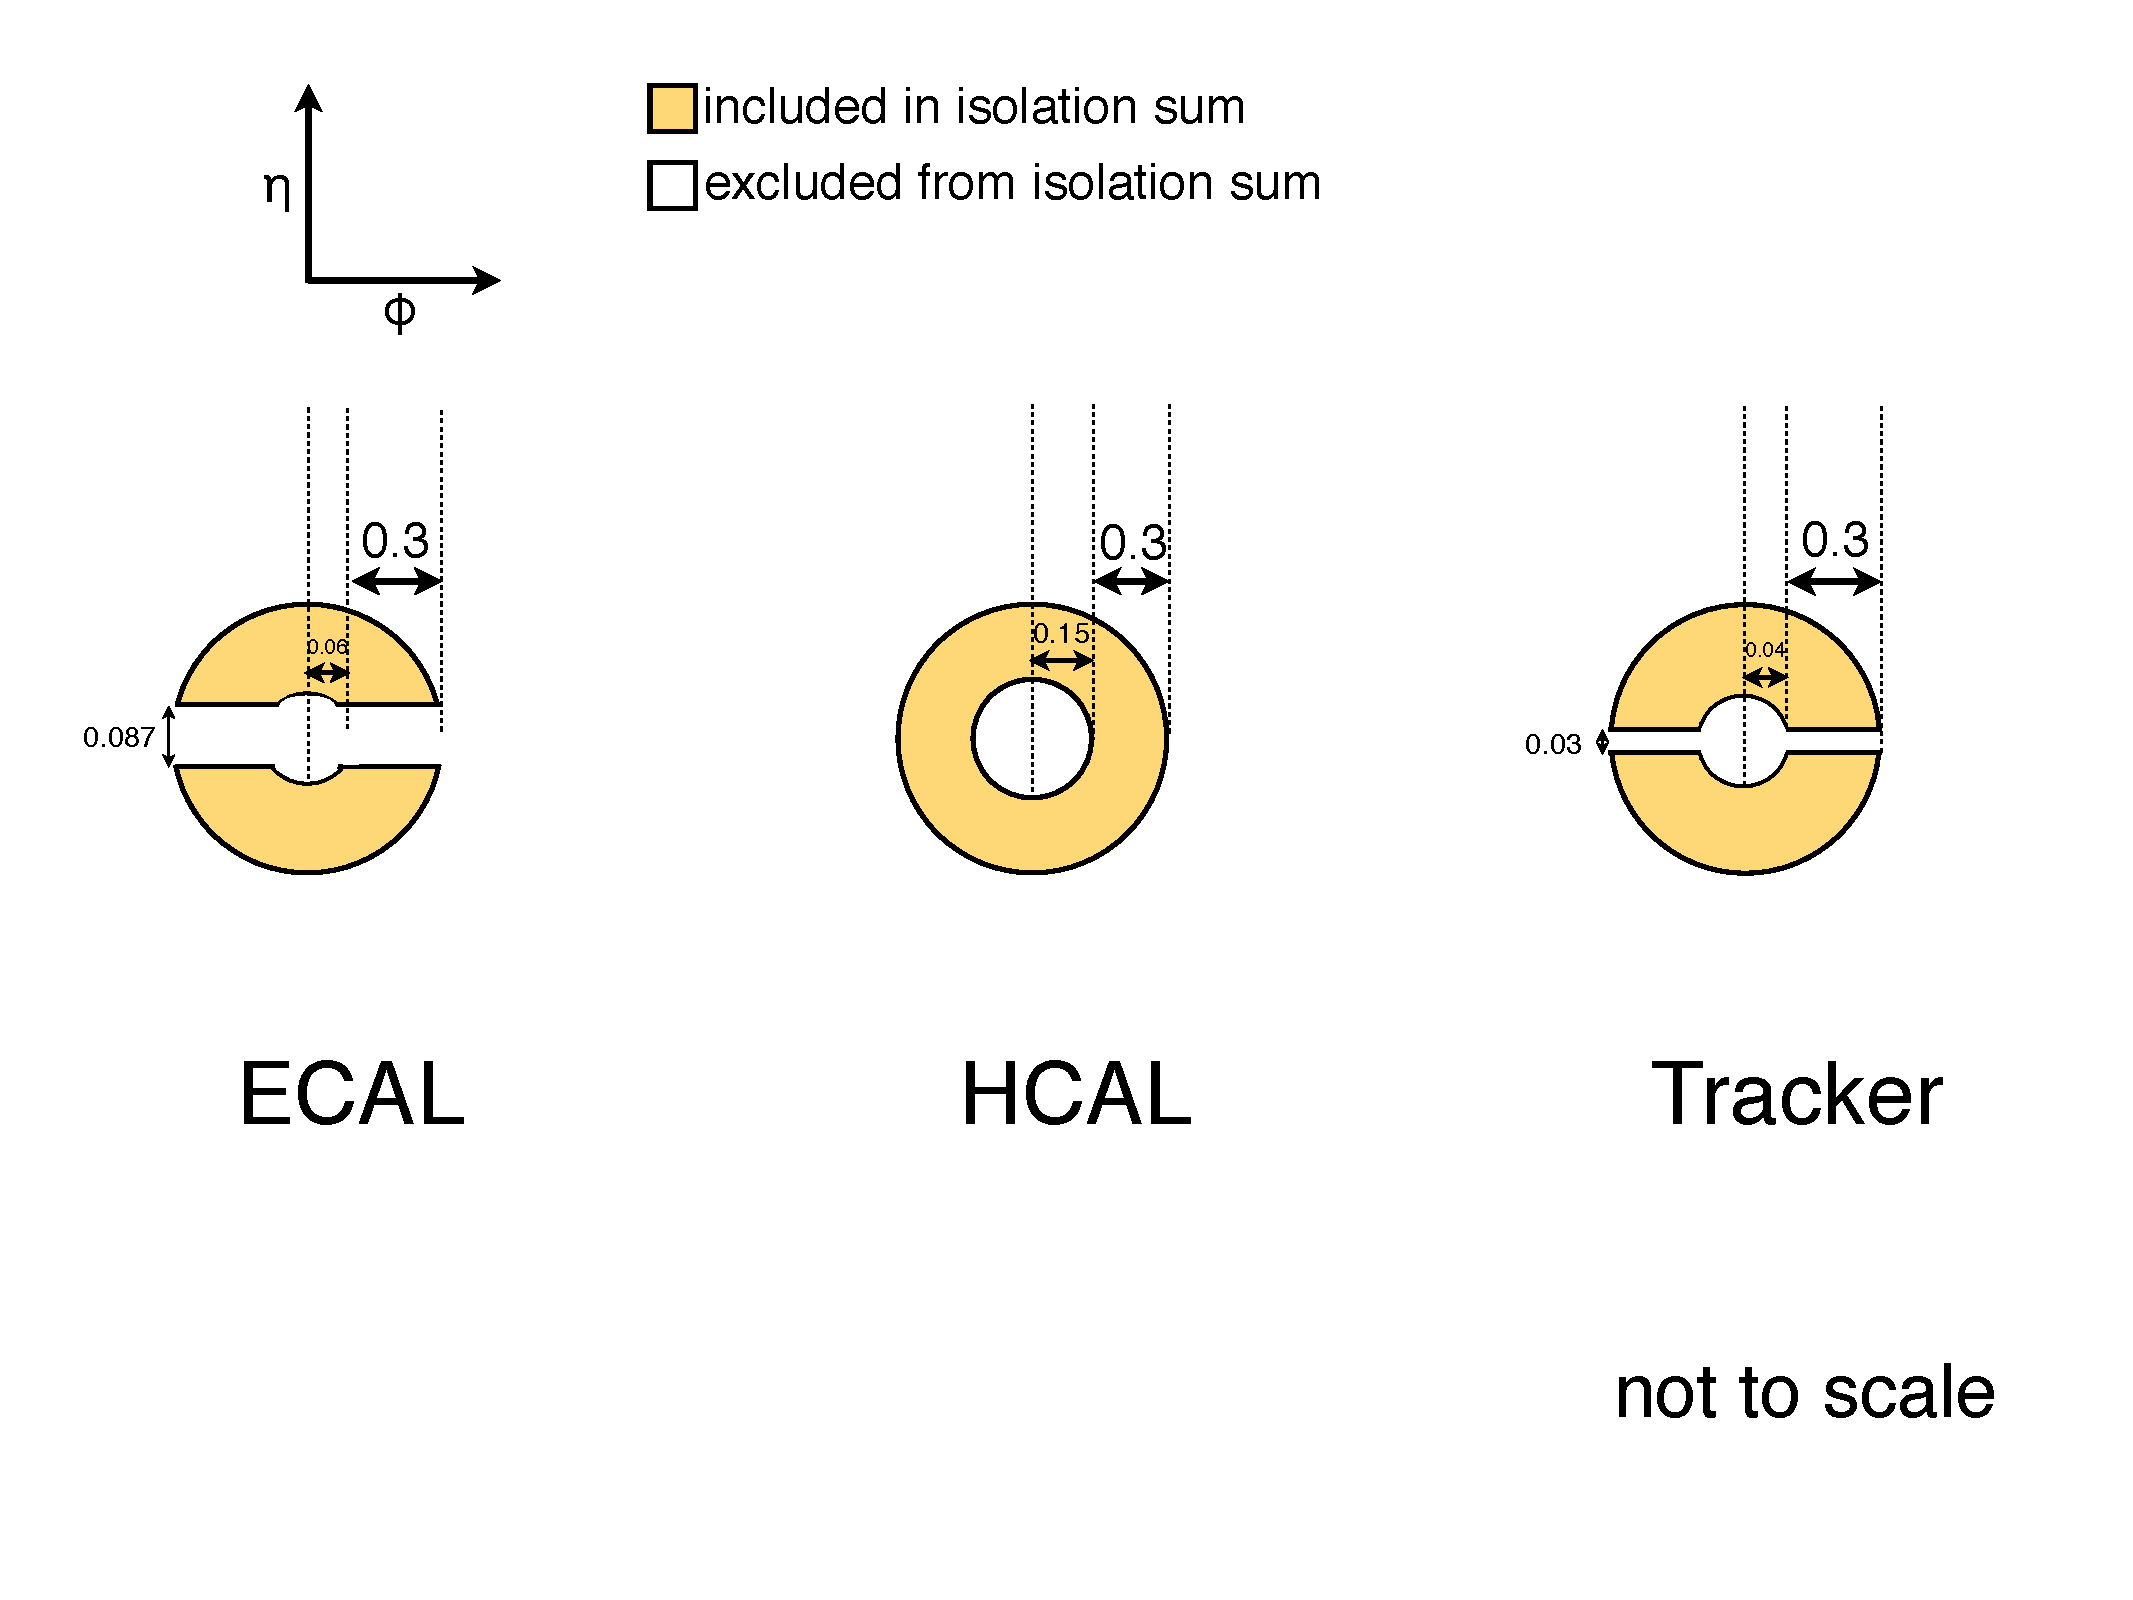
\includegraphics[scale=0.25]{isolation_cones}
	\caption{ECAL, HCAL, and track Isolation cones.}
	\label{fig:isolation_cones}
\end{figure}

\begin{figure}
	\centering
	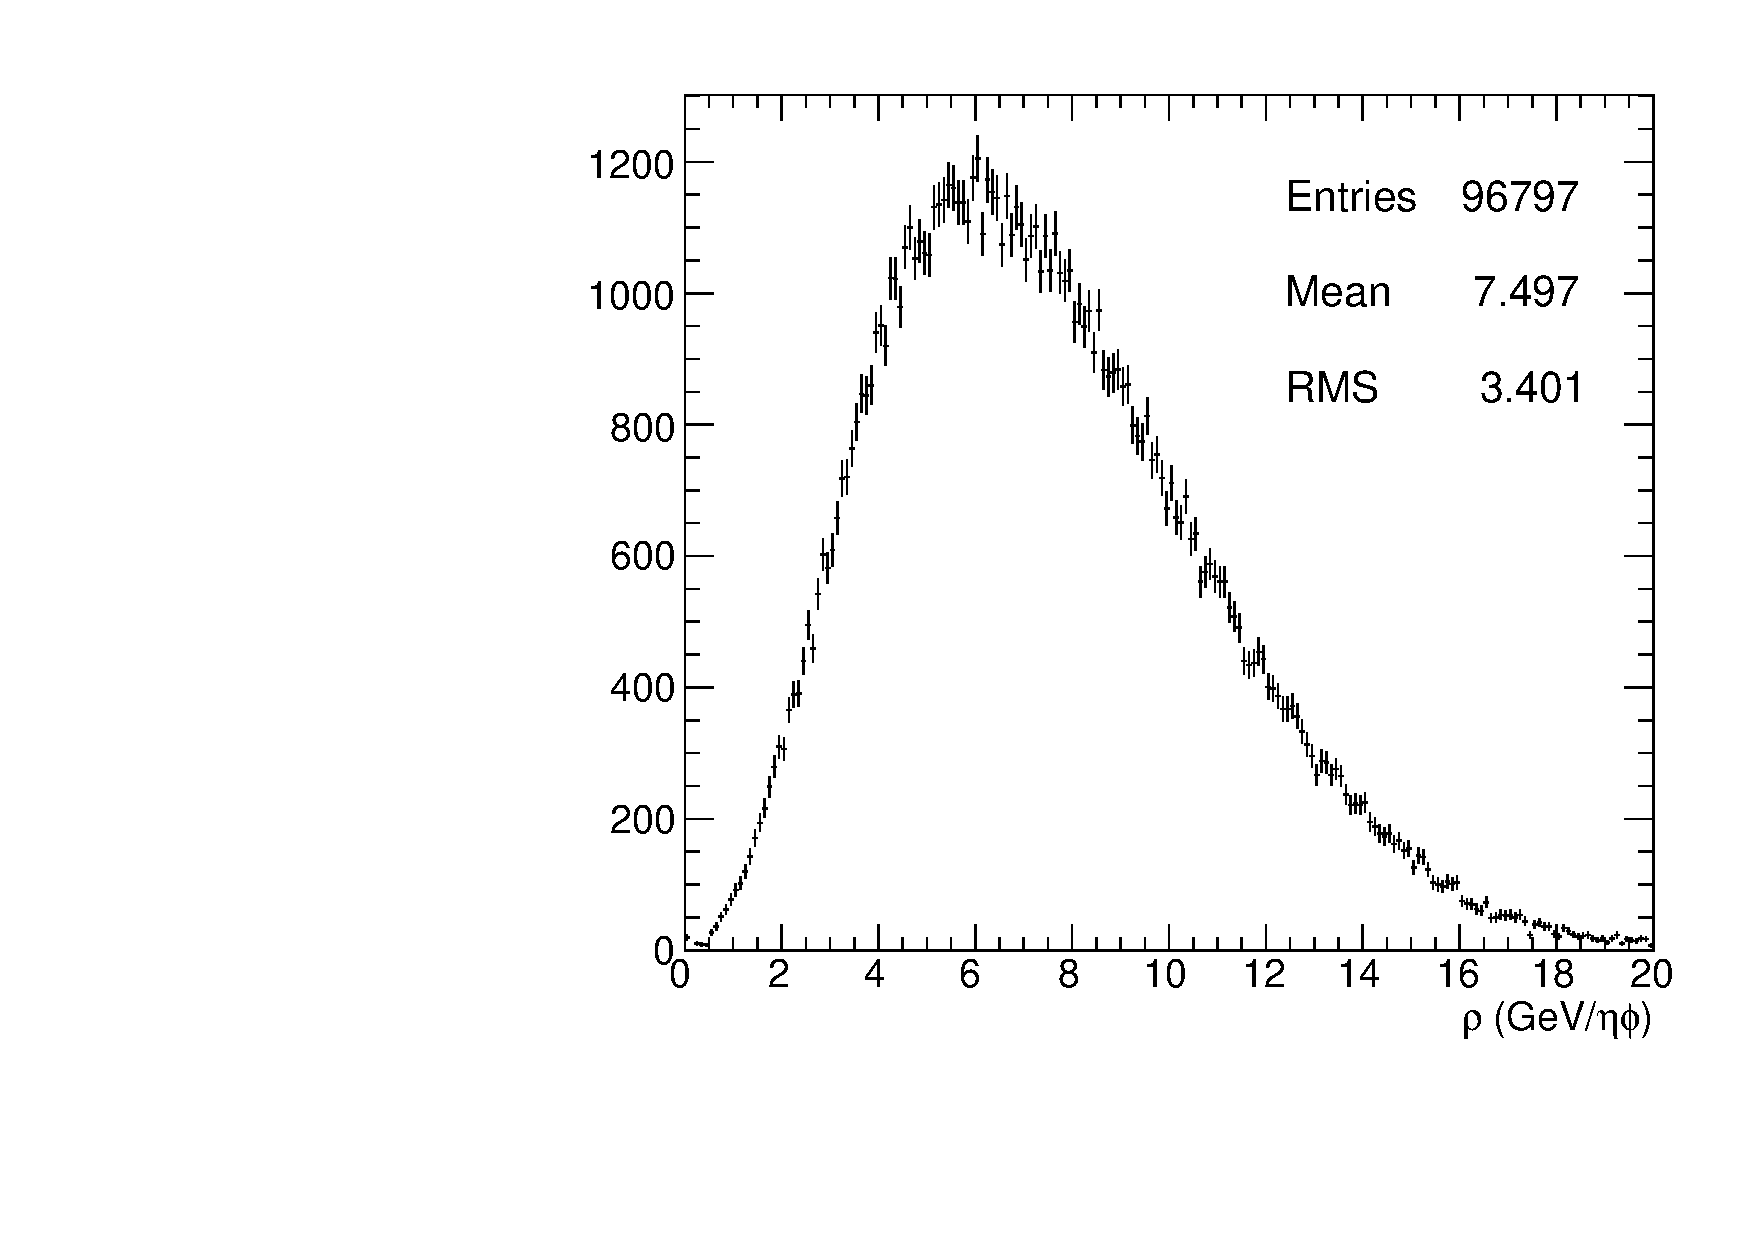
\includegraphics[scale=0.25]{preselected_rho}
	\caption{$\rho$ distribution for a sample of events with at least two 25 GeV EM objects passing the $|\eta|$, $H/E$, and $R9$ requirements in Table~\ref{g_f_criteria}, and passing the trigger requirements in Table~\ref{HLT_by_run_range}.  This sample covers the full 2011 dataset.}
	\label{fig:preselected_rho}
\end{figure}

\subsection{Electrons}
\label{sec:Electrons}

Electrons are reconstructed identically to photons, except that in the electron case the presence of a pixel seed is enforced, rather than vetoed.\footnote{In many CMS analyses, electrons are reconstructed very differently from photons.  In particular, a special tracking algorithm \cite{GSF_reco} is used to best follow a radiating electron.  However, in this analysis, the electron tracking is not used.}  Photons and electrons are defined by very similar criteria so that $Z\rightarrow ee$ events can be used to model the QCD background in the two-photon sample without introducing any bias in the electron energy measurement (cf. Sec.~\ref{sec:Modeling the QCD Background}).

\subsection{Jets and Missing Transverse Energy}
\label{sec:Jets and Missing Transverse Energy}

\subsubsection{Particle Flow}
\label{sec:Particle Flow}

In this analysis, jets and \MET are formed from \textit{particle flow} (PF) candidates.  The particle flow algorithm \cite{PF_algo, PF_perf} uses information from all CMS subdetectors to reconstruct as accurately as possible the positions and momenta of all visible jet constituents, exploiting the fine granularity of the tracker and ECAL to achieve a greatly improved momentum resolution over calorimeter-only jets \cite{CMS_JES_paper}.  The PF algorithm is summarized below \cite{PF_note}.

\begin{enumerate}
\item Reconstruct the fundamental detector objects via iterative procedures
\begin{itemize}
\item Tracks in the inner silicon layers
\begin{itemize}
\item High efficiency and low fake rate for charged hadrons in jets
\item Relaxed primary vertex constraint allows photon conversions, particles originating from nuclear interactions in the silicon, and long-lived particles to be reconstructed
\end{itemize}
\item Calorimeter clusters
\item Muon tracks in the outer muon layers
\end{itemize}
\item Create a ``block" of linked fundamental objects
\begin{itemize}
\item Link silicon tracks to calorimeter clusters via $\Delta R_{\mathrm{track-cluster}}$ (account for electron bremsstrahlung)
\item Link clusters in one calorimeter layer to clusters in a separate layer via $\Delta R_{\mathrm{cluster-cluster}}$
\item Link silicon tracks to muon tracks via global track $\chi^{2}$
\end{itemize}
\item ID the particles in the block
\begin{itemize}
\item If global (silicon + muon layers) muon $p_{T}$ is compatible with silicon track $p_{T}$, ID as a muon and remove corresponding tracks from block
\item ID electron tracks via special algorithm and removed all corresponding tracks and cluster from block
\item Remove fake tracks from the block
\item Remove excess track-cluster links via $\Delta R){\mathrm{track-cluster}}$ minimization (but allow multiple tracks to be associated to one cluster)
\item If the cluster energy is significantly larger then the energy of the linked track, ID as a PF photon or PF neutral hadron and remove corresponding clusters from the block
\item If the cluster is not linked to a track, ID as a PF photon or PF neutral hadron and remove corresponding clusters from the block
\item Remaining track-cluster links are PF charged hadrons
\end{itemize}
\end{enumerate}

\subsubsection{Jets}
\label{sec:Jets}

%description of the AK5 algorithm, illustration of the AK5 algorithm
PF candidates are clustered into jets by means of the anti-$k_{T}$ algorithm with $R = 0.5$ \cite{AK5}.  In this algorithm, all possible pairs of PF candidates $i, j$ are looped over, and the momenta of the pair that minimizes the ``distance" variable

\begin{eqnarray}
d_{ij} = \frac{\Delta R_{ij}^{2}}{\max(k_{Ti}^{2}, k_{Tj}^{2})}
\end{eqnarray}
%what is kTi?
are combined, where $k_{Ti}$ is the ?????????.  The constituent PF candidates are clustered together.  The process is repeated until $d_{ij} > R$ for all pairs of clustered PF momenta, where $R = 0.5$ \cite{Salam_talk}.  An illustration is given in Figure~\ref{fig:anti-kT}.  The anti-$k_{T}$ algorithm is infrared and collinear safe, leading to well-behaved theoretical predictions and ease of comparison between data and MC simulation.  It also tends to form circular jets, making it easy for experimental effects such as expected out-of-cone energy and fiducial acceptance to be measured or simulated.  For these reasons, the anti-$k_{T}$ jet clustering algorithm was chosen for this analysis.

\begin{figure}
	\centering
	\includegraphics[scale=0.25]{anti-kT}
	\caption{Example event display showing jets clustered via the anti-$k_{T}$ algorithm.  y is pseudorapidity.}
	\label{fig:isolation_cones}
\end{figure}

%non-compensation: e/h > 1 due to very different EM and hadronic calorimeter technologies and intrinsic losses in overcoming nuclear binding energy during strong interactions (cite Wigmans)
%sampling fluctuations

Once jets are clustered, they must be corrected due for the highly non-compensating nature of the CMS calorimeter.

%corrected for pileup and UE (L1), relative response vs. eta (L2), absolute response vs. ET (L3)
%full correction procedure, level by level
%see JES paper for details and plots
%explain sources of uncertainty in each method

\section{HLT}
\label{sec:HLT}

From the objects described in Sec.~\ref{sec:Object Reconstruction}, four samples of events are formed:

\begin{itemize}
\item $\gamma\gamma$ candidate sample, in which the two highest $E_{T}$ objects are photons,
\item $e\gamma$ control sample, in which the two highest $E_{T}$ objects are one electron and one photon,
\item $ee$ control sample, in which the two highest $E_{T}$ objects are electrons, and
\item $\mathit{ff}$ control sample, in which the two highest $E_{T}$ objects are fakes.
\end{itemize}
%
In all samples, the leading EM object is required to have $E_{T} > 40$ GeV, while the trailing EM object is required to have $E_{T} > 25$ GeV.  The high level triggers used to select the four samples, by run range, are listed in Table~\ref{tab:HLT_by_run_range}.  No trigger is prescaled.

%center the sample names?
\begin{table}[hcbp]
\caption{HLT paths triggered by the $\gamma\gamma\mbox{, }e\gamma\mbox{, }ee\mbox{, and }\mathit{ff}$ samples, by run range.  No triggers are prescaled.}
\centering
\begin{tabular}{|c|m{2.6cm}|m{2.6cm}|m{2.6cm}|m{2.6cm}|}
\hline
Run range & $\gamma\gamma$ & $e\gamma$ & $ee$ & $\mathit{ff}$ \\
\hline
\hline
160404-161215 & Photon26\_\newline IsoVL\_\newline Photon18 & Photon26\_\newline IsoVL\_\newline Photon18 & Photon26\_\newline IsoVL\_\newline Photon18 & Photon26\_\newline IsoVL\_\newline Photon18 \\
\hline
161216-166346 & Photon36\_\newline CaloIdL\_\newline Photon22\_\newline CaloIdL &  Photon36\_\newline CaloIdL\_\newline Photon22\_\newline CaloIdL &  Photon36\_\newline CaloIdL\_\newline Photon22\_\newline CaloIdL &  Photon36\_\newline CaloIdL\_\newline Photon22\_\newline CaloIdL \\
\hline
166347-180252 & Photon36\_\newline CaloIdL\_\newline IsoVL\_\newline Photon22\_\newline CaloIdL\_\newline IsoVL & Photon36\_\newline CaloIdL\_\newline IsoVL\_\newline Photon22\_\newline CaloIdL\_\newline IsoVL & Photon36\_\newline CaloIdL\_\newline IsoVL\_\newline Photon22\_\newline CaloIdL\_\newline IsoVL\newline\newline Photon36\_\newline CaloIdL\_\newline IsoVL\_\newline Photon22\_\newline R9Id\newline\newline Photon36\_\newline R9Id\_\newline Photon22\_\newline CaloIdL\_\newline IsoVL\newline\newline Photon36\_\newline R9Id\_\newline Photon22\_\newline R9Id & Photon36\_\newline CaloIdL\_\newline IsoVL\_\newline Photon22\_\newline CaloIdL\_\newline IsoVL\newline\newline Photon36\_\newline CaloIdL\_\newline IsoVL\_\newline Photon22\_\newline R9Id\newline\newline Photon36\_\newline R9Id\_\newline Photon22\_\newline CaloIdL\_\newline IsoVL\newline\newline Photon36\_\newline R9Id\_\newline Photon22\_\newline R9Id \\
\hline
\end{tabular}
\label{tab:HLT_by_run_range}
\end{table}

Each piece of the HLT path name is defined as follows.

\begin{itemize}
\item ``Photon": Energy deposit in the ECAL that fired an L1 trigger (cf. Sec.~\ref{sec:Level 1 and High Level Trigger Systems}).  For Photon26\_IsoVL\_Photon18, the L1 seed $E_{T}$ threshold is 12 GeV, while for all other triggers in Table~\ref{tab:HLT_by_run_range} it is 20 GeV.  %how is L1 energy computed?
\item Integer following the word ``Photon": $E_{T}$ threshold in GeV for offline reconstructed photon, using the full photon reconstruction of Sec.~\ref{sec:Photons} minus the laser calibrations and assuming the primary vertex at (0, 0, 0).
\item ``CaloIdL": For EB photons, $H/E < 0.15$ and $\sigma_{i\eta i\eta} < 0.014$.
\item ``IsoVL": $I_{\mathrm{ECAL}} < 0.012E_{T} + 6$ GeV, $I_{\mathrm{HCAL}} < 0.005E_{T} + 4$ GeV, and $I_{\mathrm{track}} < 0.002E_{T} + 4$ GeV.
\item ``R9Id": $R9 > 0.8$.
\end{itemize}
%
In addition, the versions of HLT\_Photon26\_IsoVL\_Photon18 and \\Photon36\_CaloIdL\_Photon22\_CaloIdL that were active during runs 160404-163268 included a cut $E_{\mathrm{max}}/E_{5\times 5} < 0.98$ for spike rejection.  $E_{\mathrm{max}}$ is the energy in the highest energy crystal of the EM cluster and $E_{5\times 5}$ is the energy in the 5$\times$5 crystal matrix around the seed crystal.  For runs after 163268, Swiss cross spike rejection of individual crystals from HLT quantities was performed (cf. Sec.~\ref{Photons}).  All information about the evolution of the CMS HLT settings can be found in the HLT configuration browser at \url{http://j2eeps.cern.ch/cms-project-confdb-hltdev/browser/}.

As an example of the naming convention just described, the HLT path Photon36\_CaloIdL\_IsoVL\_Photon22\_R9Id is fired if one photon is found with $E_{T} > 36$ GeV passing the CaloIdL and IsoVL requirements, and another is found with $E_{T} > 22$ GeV passing the R9Id requirement.

\section{Photon Identification Efficiency}
\label{sec:Photon Identification Efficiency}

Lorum ipsum fuck Republicans.

\end{document}